\chapter{Introducción}
\label{cap:Introduccion}
El consumo de energía juega un papel muy importante en el progreso y bienestar de la sociedad. Tanto es así, que la demanda energética no deja de crecer, por ello deben llevarse a cabo medidas para reducir el consumo elevado de energía, lo que se conoce como eficiencia energética. La eficiencia energética~\cite{GarSa12} se refiere a medios de optimización en la producción y en medios de aprovechamiento en su uso. \\
Por otro lado, puesto que las fuentes de energía fósil y nuclear son finitas, podría llegar el día en el que no se pueda satisfacer la demanda energética, salvo que se apueste por los métodos alternativos de obtención de energía. Es aquí donde entran en juego las energías renovables. Una de ellas es la energía solar~\cite{Perp12}, que permite el aprovechamiento de la radiación electromagnética del sol. Entre las aplicaciones más comunes de la energía solar fotovoltaica se encuentra la producción de energía eléctrica para su inyección en la red eléctrica (mercado eléctrico), abordada en este trabajo fin de grado. \\


Teniendo en cuenta estos dos antecedentes, existe una motivación a la hora de obtener la energía demandada de la forma mas óptima y limpia posible. Este trabajo se centrará en la creación de un \textbf{sistema inteligente} para la gestión de energía de una infraestructura fotovoltaica desde el punto de vista de una empresa distribuidora. En función de un escenario determinado (situación meteorológica, precio del kilovatio-hora (kwh) en el mercado eléctrico, nivel de carga de las baterías de almacenaje, etc) se modelará la cantidad de potencia eléctrica recibida por cada una de las entradas. De igual modo, se modelará la cantidad de potencia eléctrica suministrada a cada una de las salidas. Esto se traduce en una optimización y aprovechamiento de la energía.
En la Figura 1 se muestra un esquema del sistema donde se identifican desde un alto nivel de abstracción las entradas y salidas.\\

\begin{figure}[!h]
	\centering
	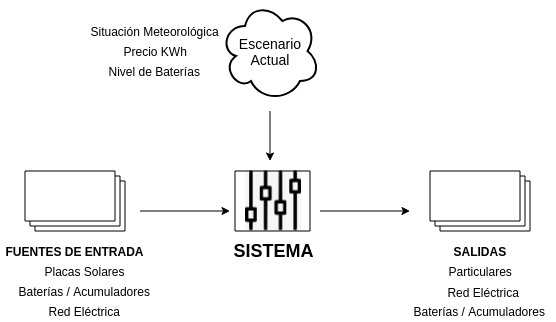
\includegraphics[width=10cm]{figs/Abstract.png}
	\caption{Esquema del sistema}
\end{figure}
